\subsection{Terzo tutorial: Dependency Management}
Una delle parti più importanti di uno strumento di questo tipo è la gestione delle dipendenze che si divide in 2 parti: incoming files e outgoing files. Infatti Gradle ha bisogno di conoscere di cosa il nostro progetto ha bisogno per poter essere compilato ed eseguito, queste vengono chiamate dipendenze (dipendencies) che in questo caso sono gli incoming files. Gli outgoing files sono invece tutto ciò che il tuo progetto produce chiamati anche pubblicazioni (pubblications). Il Dependency Manager di Gradle permette di scaricare le dipendenze del progetto da diversi remote repository specificando direttamente il nome e la versione della dipendenza voluta.

\subsubsection{Dichiarazione delle dipendenze}
Prima di tutto è necessario indicare in che linguaggio il nostro progetto viene rilasciato (consideriamo d'ora in poi solo il caso di Java), per farlo aggiungiamo in testa al file build.gradle:
\begin{verbatim}
apply plugin: 'java' \end{verbatim}
A questo punto per poter usufruire di una dipendenza è necessario specificare da dove Gradle deve andare a prenderla, dobbiamo quindi indicare il repository remoto di riferimento. Se per esempio vogliamo che il nostro repository di riferimento sia Maven allora dobbiamo aggiungere al build.gradle:
\begin{verbatim}
repositories {
    mavenCentral()
} \end{verbatim}
In questo modo tutte le dipendenze che andremo a indicare successivamente saranno riferimenti alle pubblicazioni su MavenCentral. La dichiarazione delle dipendenze deve essere inserita nel tag \texttt{dependencies} nel build.gradle file, per esempio vogliamo avere junit 4.12 come dipendenza al nostro progetto Gradle allora dobbiamo aggiungere:
\begin{verbatim}
dependencies {
    testCompile group: 'junit', name: 'junit', version: '4.12' 
} \end{verbatim}
osserviamo che nella dichiarazione ci sono 4 diversi indicatori:
\begin{itemize}
    \item \texttt{testCompile} indica a che tipo di build deve fare riferimento, in questo caso questa dipendenza sarà importata durante la compilazione dei test;
    \item \texttt{group, name, version} corrispondono rispettivamente al groupId, artifactId e al version definiti su Maven.
\end{itemize}
esiste un modo molto più diretto per indicare una dipendenza, considerando sempre la dipendenza junit possiamo scrivere:
\begin{verbatim}
dependencies {
    testCompile 'junit:junit:4.12'
} \end{verbatim}
ha lo stesso significato precedente ma ha una forma più compatta, forma che adotta anche la documentazione Maven.
\begin{figure}[H]
\centering
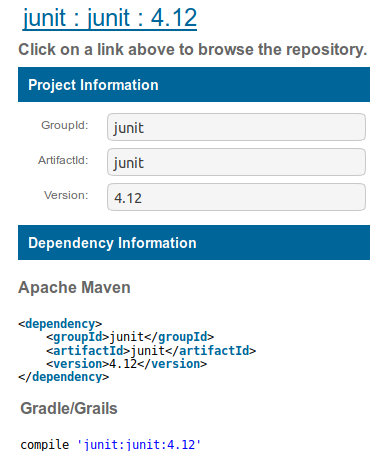
\includegraphics[width=0.4\linewidth]{Tutorial/third/gradleInMavenRepo.png}
\end{figure} 
Possiamo notare ora la differenza sostanziale della configurazione delle dipendenze tra il pom.xml di Maven e la build.gradle di Gradle. A questo punto possiamo scaricare le dipendenze, per farlo eseguiamo il comando gradle (usando il wrapper): 
\begin{verbatim}
    $ ./gradlew dependencies \end{verbatim}
L'output restituirà la lista di tutti i task con le relative dipendenze (se ce ne sono), nel caso la dipendenza richiesta non si trova nel progetto provvederà a scaricarla.